\documentclass[aspectratio=169]{beamer}

\usetheme{Boadilla}
\usecolortheme{beaver}
\setbeamertemplate{navigation symbols}{}
\setbeamertemplate{footline}[frame number]

\usepackage[utf8]{inputenc}
\usepackage[brazil]{babel}
\usepackage{booktabs}
\usepackage{graphicx}
\usepackage{amsmath}
\usepackage{multirow}
\usepackage{xcolor}

\definecolor{gain}{RGB}{0,128,0}
\definecolor{loss}{RGB}{180,0,0}

\title[Avaliação Semântica de SR]{Avaliação Semântica de Super-Resolução Temporal\\em Imagens Sentinel-2 por Métricas de PLN}
\author{Marcel Fernandes Gomes}
\institute{PPGC -- UFRGS \\ CMP617 -- Processamento de Linguagem Natural e Recuperação de Informações}
\date{10 de junho de 2026}

% ============================================================
\begin{document}
% ============================================================

\begin{frame}
  \titlepage
\end{frame}

% ----------------------------------------------------------
\begin{frame}{Motivação: o que muda quando aumentamos a resolução?}

  \begin{columns}[T]
    \begin{column}{0.55\textwidth}
      \begin{itemize}
        \item Sentinel-2: cobertura global, mas $\approx$10\,m/px\\
              $\Rightarrow$ limita feições finas (bordas de campo, corpos d'água pequenos, estradas vicinais.)
        \item Super-resolução (SR) temporal: fusão de múltiplas observações\\
              $\Rightarrow$ $\approx$2{,}5\,m/px
        \item PSNR/SSIM são métricas clássicas que avaliam apenas valores numéricos de \textit{pixels}, e não significado.
      \end{itemize}
      \begin{block}{Problema central}
      	Como saber se o conteúdo recuperado é \emph{semanticamente correto}?
      \end{block}
    \end{column}
    \begin{column}{0.42\textwidth}
      \centering
      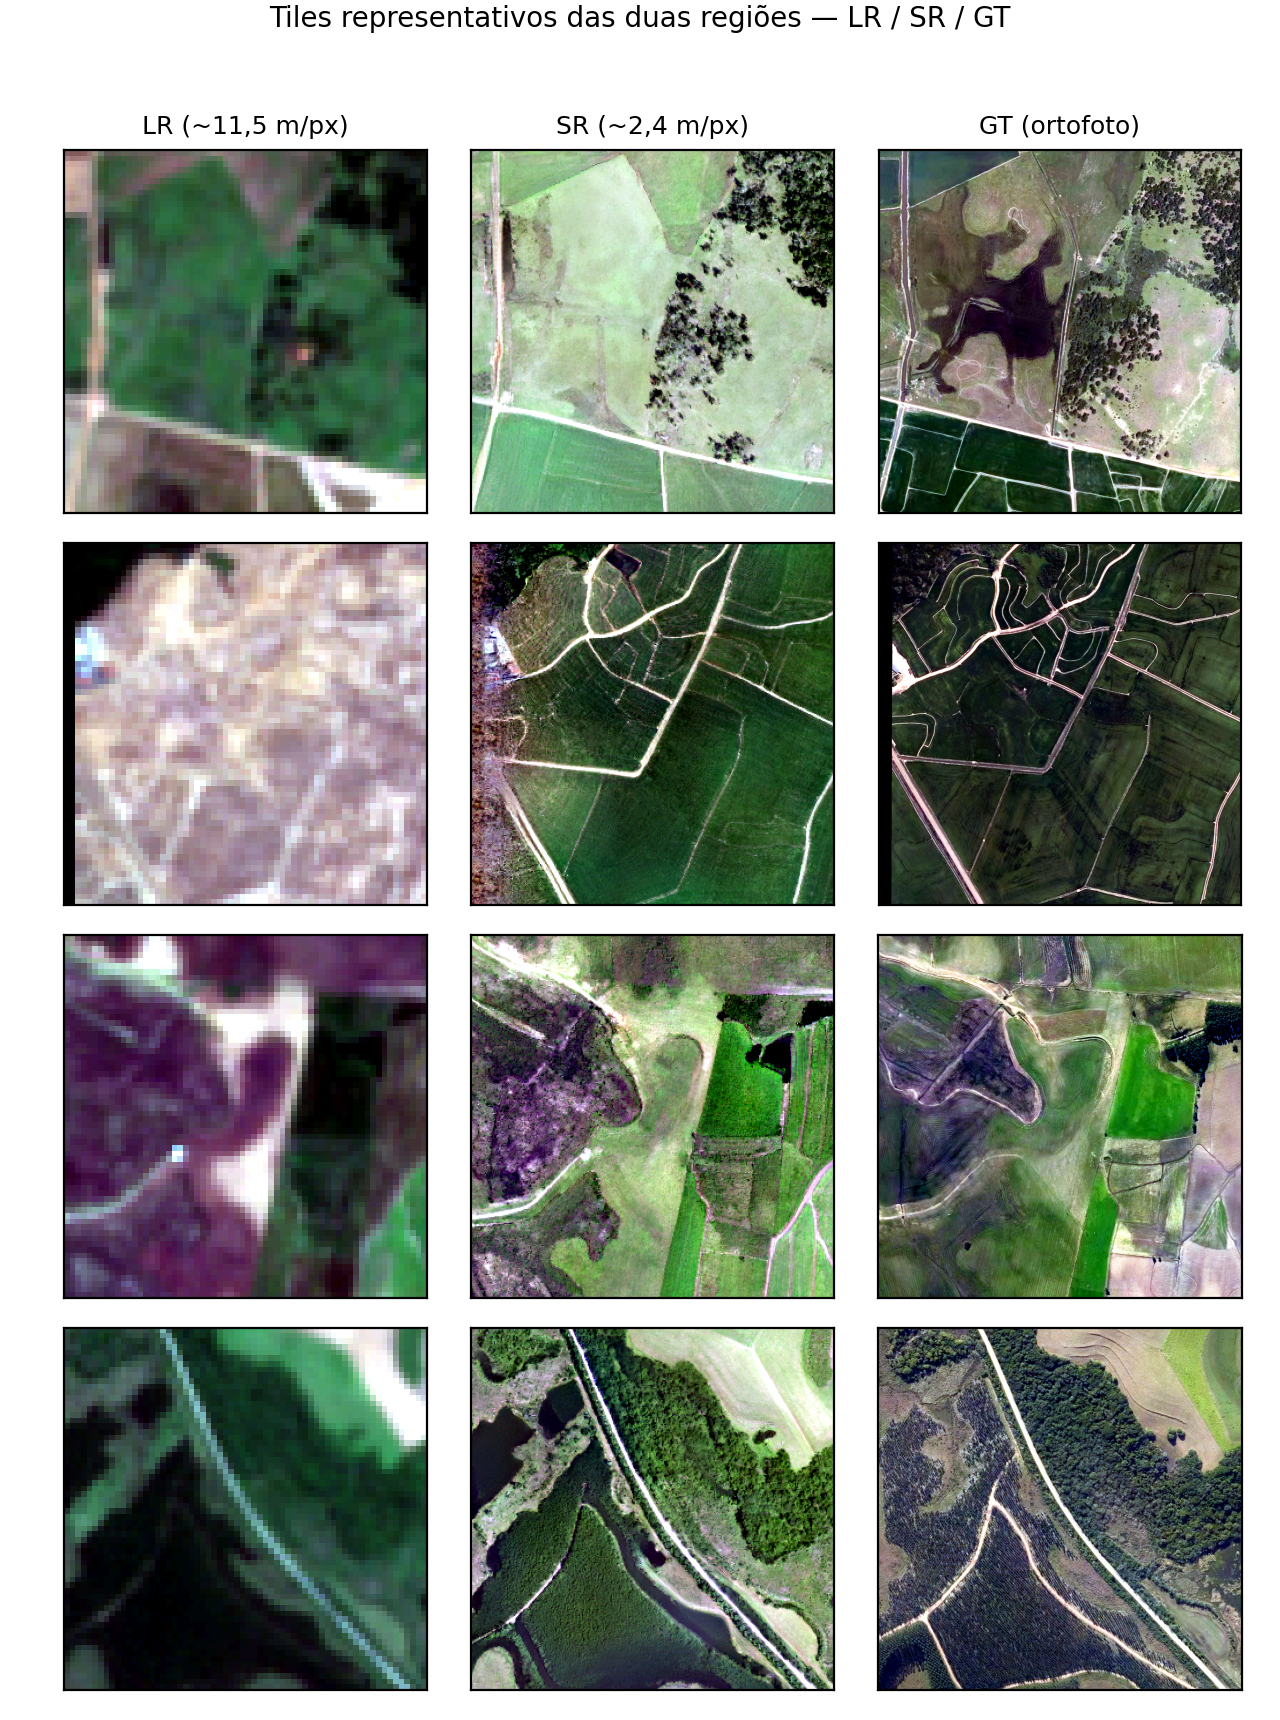
\includegraphics[width=\linewidth,height=0.62\textheight,keepaspectratio]{figures/fig_grid_representativo.png}\\
      {\small LR \quad\quad SR \quad\quad GT}
    \end{column}
  \end{columns}

\end{frame}

% ----------------------------------------------------------
\begin{frame}{Proposta: pipeline de avaliação semântica}

  \begin{block}{Ideia central}
    Usar modelos visão-linguagem para \emph{descrever} as imagens LR e SR
    e comparar as descrições com referências conhecidas — sem par HR alinhado.
  \end{block}

  \vspace{0.5em}
  \textbf{Três eixos de avaliação:}

  \begin{enumerate}
    \item \textbf{NLP (texto $\leftrightarrow$ texto):} BLIP/GeoChat geram legendas $\to$ BLEU-1, ROUGE-1, TF-IDF
    \item \textbf{CLIPScore (imagem $\leftrightarrow$ imagem):} embeddings CLIP e RemoteCLIP comparam SR e GT
    \item \textbf{VQA estratificada:} GeoChat responde 7 perguntas objetivas em 3 níveis
  \end{enumerate}

  \vspace{0.5em}
  \textbf{Contribuição central:} avaliação cruzada VQA × GeoPackage\\
  $\rightarrow$ estima cobertura do solo, compara com GT vetorial em pontos percentuais (pp)

  \vspace{0.3em}
  \textit{Validação: pipeline replicado em duas regiões geográficas distintas ($n=953$ tiles).}

\end{frame}

% ----------------------------------------------------------
\begin{frame}{Dados e configuração experimental}

  \begin{columns}[T]
    \begin{column}{0.50\textwidth}
      \textbf{Imagens — Sul do Brasil}
      \begin{itemize}
        \item \textbf{LR:} Sentinel-2 nativo, $\approx$11{,}5\,m/px (distorção ao afastar da Linha do Equador)
        \item \textbf{SR:} fusão temporal de 8 obs., $\approx$2{,}5\,m/px
        \item \textbf{GT raster:} ortofoto aérea, $\approx$1\,m/px
        \item \textbf{GT vetorial:} GeoPackage com 7 classes de cobertura do solo
      \end{itemize}
      \vspace{0.4em}
      \textbf{Tiling:} grade 64×64\,px no espaço LR ($\approx$0{,}73\,km²/tile)
    \end{column}
    \begin{column}{0.47\textwidth}
      \textbf{Duas regiões ($\approx$110\,km entre si):}
      \vspace{0.2em}
      \begin{tabular}{lrr}
        \toprule
        & \textbf{R1} & \textbf{R2} \\
        \midrule
        Tiles válidos & 575 & 378 \\
        Paisagem & mista & agrícola \\
        Água & frequente & rara \\
        \midrule
        \textbf{Total} & \multicolumn{2}{c}{\textbf{953 tiles}} \\
        \bottomrule
      \end{tabular}
      \vspace{0.4em}

      \textbf{Cenários de referência:}
      \begin{itemize}\small
        \item \textbf{A:} nome da classe vetorial
        \item \textbf{B:} legenda/embedding da ortofoto
        \item \textbf{C:} igual a B, GT reamostrado para SR
      \end{itemize}
    \end{column}
  \end{columns}

\end{frame}

% ----------------------------------------------------------
\begin{frame}{Eixo 1 — NLP com BLIP: alucinações e limitação léxica}

  \textbf{Cenário A (GT = nome da classe):} scores próximos de zero em ambas resoluções
  \begin{itemize}
    \item BLIP raramente reproduz literalmente "forest", "bare ground", etc.
    \item \textbf{Mas revela algo importante sobre a LR:}
  \end{itemize}

  \vspace{0.3em}
  \begin{block}{20\% dos tiles LR geram alucinações}
    \textit{``a blue sky with clouds''}, \textit{``a couple is kissing in the water''}\\
    $\Rightarrow$ baixa resolução leva o BLIP a evocar cenas do pré-treinamento\\
    SR reduz esse colapso de \textbf{20\%} para \textbf{11\%} dos tiles
  \end{block}

  \vspace{0.4em}
  \textbf{Cenário B (GT = legenda da ortofoto):} resultado mais limpo
  \begin{itemize}
    \item TF-IDF (pooled): LR $= 0{,}079$ \quad SR $= 0{,}279$ \quad $\Delta = +0{,}201$
    \item Favorável à SR em 685/953 tiles (pooled)
  \end{itemize}

  \vspace{0.3em}
  \small\textit{Limitação: BLIP infla o gap porque colapsa na LR. Motiva o uso do GeoChat.}

\end{frame}

% ----------------------------------------------------------
\begin{frame}{Eixo 2 — CLIPScore imagem-imagem}

  \begin{center}
    \textbf{RemoteCLIP mede diretamente: a SR é mais parecida com a ortofoto?}
  \end{center}

  \vspace{0.3em}
  \begin{columns}[T]
    \begin{column}{0.50\textwidth}
      \begin{tabular}{lccc}
        \toprule
        \textbf{Modelo} & \textbf{Região} & $\mathbf{\Delta}$ & \textbf{SR${>}$LR} \\
        \midrule
        \multirow{3}{*}{CLIP gen.}
          & R1     & $+0{,}356$ & 562/575 \\
          & R2     & $+0{,}345$ & 368/378 \\
          & pooled & $+0{,}352$ & 930/953 \\
        \midrule
        \multirow{3}{*}{\textbf{RemoteCLIP}}
          & R1     & $+0{,}505$ & 574/575 \\
          & R2     & $+0{,}512$ & 378/378 \\
          & \textbf{pooled} & $\mathbf{+0{,}508}$ & \textbf{952/953} \\
        \bottomrule
      \end{tabular}
    \end{column}
    \begin{column}{0.46\textwidth}
      \begin{itemize}
        \item RemoteCLIP (fine-tuned em SR) é mais sensível que CLIP genérico
        \item Resultado mais estável entre regiões de todos os eixos
        \item Diferença SR\,$>$\,LR significativa (teste de sinais, $p<0{,}001$)
        \item Cenário C (GT reamostrado): gap cai de $+0{,}508$ para $+0{,}421$\\
              $\Rightarrow$ parte da vantagem é resolução diferencial, mas hierarquia LR\,$<$\,SR persiste
      \end{itemize}
    \end{column}
  \end{columns}

\end{frame}

% ----------------------------------------------------------
\begin{frame}{Eixo 3 — VQA estratificada com GeoChat}

  \textbf{GeoChat-7B:} modelo visão-linguagem ajustado em 318\,mil pares geoespaciais\\
  $\Rightarrow$ descreve bem baixa e super-resolução --- gap menor que BLIP confirma que o ganho é real

  \vspace{0.3em}
  \begin{columns}[T]
    \begin{column}{0.57\textwidth}
      \fontsize{7.2pt}{9pt}\selectfont
      \begin{tabular}{@{}lp{5.0cm}@{}}
        \toprule
        \textbf{Nível} & \textbf{Pergunta} \\
        \midrule
        \multirow{2}{*}{L1 Semântico}
          & \textit{``Estimate the percentage of each land cover type''} \\[2pt]
          & \textit{``Is there a water body visible in the image?''} \\
        \midrule
        \multirow{2}{*}{L2 Estrutural}
          & \textit{``How many distinct agricultural fields can you count?''} \\[2pt]
          & \textit{``Are crop rows or cultivation patterns visible?''} \\
        \midrule
        \multirow{3}{*}{L3 Detalhe fino}
          & \textit{``How many individual buildings are visible?''} \\[2pt]
          & \textit{``Describe the road network visible in the image''} \\[2pt]
          & \textit{``Describe the buildings visible in the image''} \\
        \bottomrule
      \end{tabular}
    \end{column}
    \begin{column}{0.40\textwidth}
      \fontsize{8pt}{10pt}\selectfont
      \begin{tabular}{@{}lcc@{}}
        \toprule
        \textbf{Nível} & \textbf{TF-IDF $\Delta$} & \textbf{Sem. $\Delta$} \\
        \midrule
        L1 Semântico    & $+0{,}228$ & $+0{,}054$ \\
        L2 Estrutural   & $+0{,}131$ & $+0{,}044$ \\
        L3 Detalhe fino & $+0{,}122$ & $+0{,}056$ \\
        \bottomrule
      \end{tabular}
      \vspace{0.4em}
      \begin{itemize}\scriptsize
        \item SR favorável em todos os níveis e regiões
        \item L2 mais fraco: contagem de campos satura em zero para ambas as resoluções
        \item L3 maior na Região~2: paisagem agrícola se beneficia mais dos detalhes finos
      \end{itemize}
    \end{column}
  \end{columns}

\end{frame}

% ----------------------------------------------------------
\begin{frame}{Contribuição central: VQA × GeoPackage}

  \begin{block}{Problema com Cenários A--C}
    Comparação textual depende de sobreposição léxica ou alinhamento de resolução.
    O que queremos: \textbf{a SR estima melhor a cobertura real do solo?}
  \end{block}

  \vspace{0.3em}
  \textbf{Método:}
  \begin{enumerate}
    \item GeoChat responde Q1: \textit{``Estimate the percentage of each land cover type''}
    \item Extraímos as porcentagens estimadas para baixa resolução, super-resolução e GT raster
    \item Calculamos o erro absoluto médio contra as porcentagens reais do GeoPackage (ground truth vetorial)
  \end{enumerate}

  \vspace{0.2em}
  $\Rightarrow$ métrica em \textbf{pontos percentuais (pp)}, diretamente interpretável,
  sem depender de léxico ou par HR alinhado

\end{frame}

% ----------------------------------------------------------
\begin{frame}{Resultado principal: MAE de cobertura LR vs.\ SR vs.\ GT}

  \begin{columns}[T]
    \begin{column}{0.52\textwidth}
      \resizebox{\linewidth}{!}{%
      \begin{tabular}{lcc|cc|cc}
        \toprule
        & \multicolumn{2}{c|}{\textbf{R1}} & \multicolumn{2}{c|}{\textbf{R2}} & \multicolumn{2}{c}{\textbf{Pooled}} \\
        \textbf{Classe} & LR & SR & LR & SR & LR & SR \\
        \midrule
        forest      & 37,1 & 36,6 & 28,8 & 23,9 & 33,8 & 31,6 \\
        agriculture & 30,4 & 26,1 & 50,1 & 41,0 & 38,3 & 31,9 \\
        urban       &  5,1 &  3,7 &  5,0 &  5,8 &  5,1 &  4,5 \\
        water       & 11,5 &  9,6 &  4,7 & 13,4 &  8,8 & 11,1 \\
        bare soil   & 29,4 & 20,2 & 24,4 & 10,3 & 27,4 & 16,4 \\
        \midrule
        \textbf{Global} & 22,7 & \textbf{19,2} & 22,6 & \textbf{18,9} & 22,7 & \textbf{19,1} \\
        GT raster   & \multicolumn{2}{c|}{17,7} & \multicolumn{2}{c|}{16,9} & \multicolumn{2}{c}{\textbf{17,4}} \\
        \bottomrule
      \end{tabular}%
      }
      \vspace{0.3em}
      {\small Menor MAE = melhor. $\Delta_\text{pooled} = +3{,}6$\,pp (LR$-$SR).}
    \end{column}
    \begin{column}{0.45\textwidth}
      \centering
      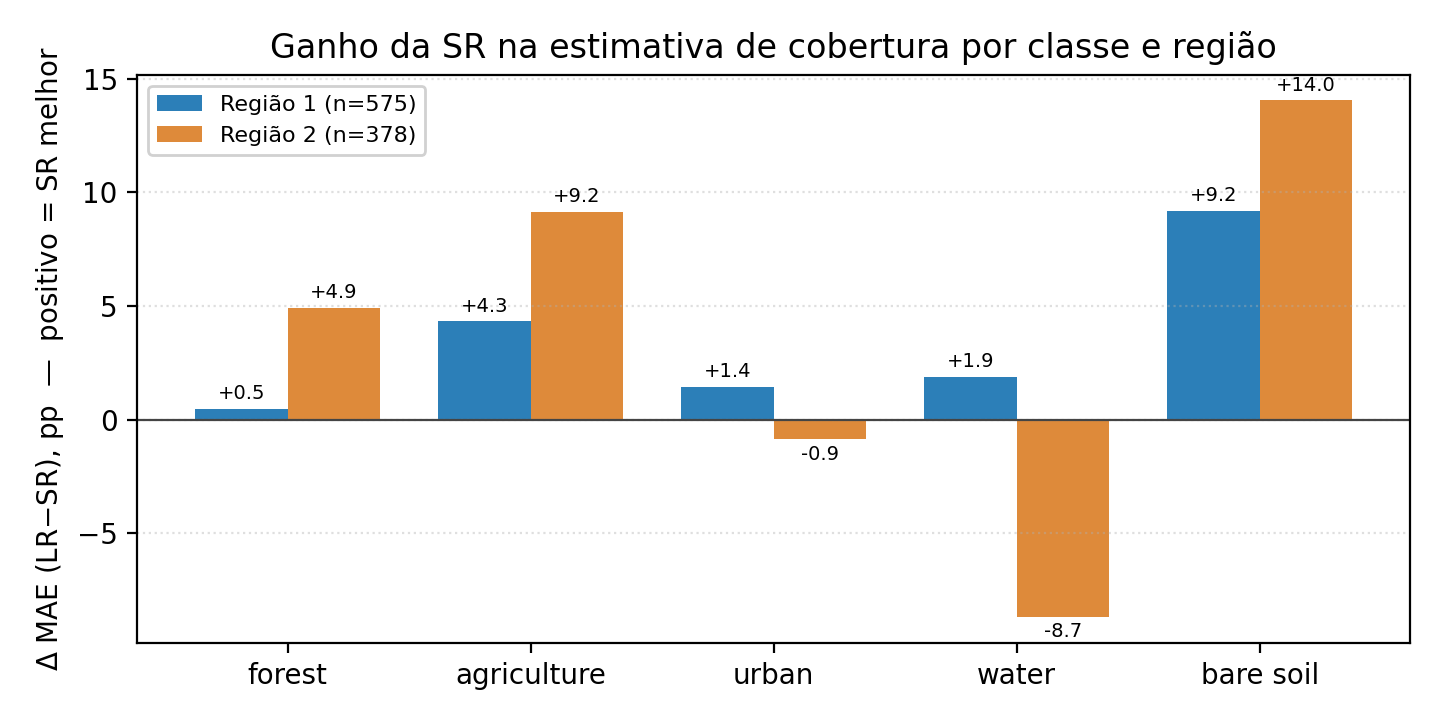
\includegraphics[width=\linewidth]{figures/fig_mae_multiregiao.png}
      {\small Ganho da SR por classe e região}
    \end{column}
  \end{columns}

\end{frame}

% ----------------------------------------------------------
\begin{frame}{Hierarquia e maiores ganhos}

  \begin{center}
    \Large
    $\underbrace{\text{GT raster}}_{\text{17,4\,pp}}$
    $\;<\;$
    $\underbrace{\text{SR}}_{\text{19,1\,pp}}$
    $\;<\;$
    $\underbrace{\text{LR}}_{\text{22,7\,pp}}$
    \normalsize\quad (MAE global pooled)
  \end{center}

  \vspace{0.4em}
  \begin{columns}[T]
    \begin{column}{0.48\textwidth}
      \textbf{Maiores ganhos (pooled):}
      \begin{itemize}
        \item \textcolor{gain}{\textbf{bare soil: $+11{,}1$\,pp}}\\
              robustos nas duas regiões (+9,2 / +14,0)
        \item \textcolor{gain}{\textbf{agriculture: $+6{,}3$\,pp}}\\
              especialmente R2 (+9,2\,pp)
      \end{itemize}
      $\Rightarrow$ fusão temporal recupera informação semântica real sobre cobertura relevante para monitoramento agrícola/ambiental
    \end{column}
    \begin{column}{0.48\textwidth}
      \textbf{Nuance: classe water}
      \begin{itemize}
        \item R1 (água frequente): SR melhora ($+1{,}9$\,pp)
        \item R2 (água rara): SR superestima ($-8{,}7$\,pp)
        \item pooled: $-2{,}3$\,pp
      \end{itemize}
      \vspace{0.2em}
      Onde a água é rara, a SR tende a superestimá-la --- lembrete de
      calibrar expectativas por tipo de paisagem.
    \end{column}
  \end{columns}

\end{frame}

% ----------------------------------------------------------
\begin{frame}{Papel da validação multi-região}

  \begin{columns}[T]
    \begin{column}{0.48\textwidth}
      \textbf{O que a multi-região confirmou:}
      \begin{itemize}
        \item Ganhos globais são consistentes (R1 $\approx$ R2 na maioria das métricas)
        \item RemoteCLIP: $+0{,}505$ / $+0{,}512$ praticamente idênticos
        \item Ganhos em bare soil e agriculture reproduzíveis
      \end{itemize}
    \end{column}
    \begin{column}{0.48\textwidth}
      \textbf{O que a multi-região \emph{revelou}:}
      \begin{itemize}
        \item Ganhos se mantêm em paisagem mais agrícola (R2)
        \item Ganho global pode coexistir com nuance por classe (ex.: \textit{water} em R2)
        \item Robustez não atestável por estudo de área única
      \end{itemize}
    \end{column}
  \end{columns}

  \vspace{0.5em}

\end{frame}

% ----------------------------------------------------------
\begin{frame}{Resumo: o que cada eixo mede}

  \begin{tabular}{p{3cm}p{4.5cm}p{5cm}}
    \toprule
    \textbf{Eixo} & \textbf{O que mede} & \textbf{Principal achado} \\
    \midrule
    BLIP NLP & Qualidade léxica das legendas & SR reduz alucinações de 20\% → 11\% \\[0.3em]
    CLIPScore RemoteCLIP & Similaridade semântica imagem-imagem & SR $>$ LR em 952/953 tiles \\[0.3em]
    GeoChat NLP & Qualidade com modelo robusto & Gap menor confirma que BLIP infla o resultado \\[0.3em]
    VQA estratificada & Informação discriminada por nível & Todos os níveis favorecem SR \\[0.3em]
    \textbf{VQA × GeoPackage} & \textbf{Erro de cobertura em pp} & \textbf{$-3{,}6$\,pp global; maior em bare soil e agriculture} \\
    \bottomrule
  \end{tabular}

\end{frame}

% ----------------------------------------------------------
\begin{frame}{Conclusão e trabalhos futuros}

  \begin{block}{Resposta à pergunta central}
    Sim: a SR por fusão temporal recupera conteúdo semântico mensurável — e o pipeline proposto quantifica esse ganho sem métricas de pixel.
  \end{block}

  \vspace{0.4em}
  \textbf{Contribuições:}
  \begin{enumerate}
    \item Pipeline semântico (NLP + CLIPScore + VQA) para avaliação de SR de satélite
    \item \textbf{Avaliação cruzada VQA × GeoPackage:} métrica quantitativa em pp, sem dependência léxica
    \item Validação multi-região que confirma robustez e expõe modo de falha (water em R2)
  \end{enumerate}

  \vspace{0.4em}
  \textbf{Trabalhos futuros:}
  \begin{itemize}
    \item Reformular perguntas VQA de nível estrutural (q03 saturou)
    \item Ampliar para mais regiões, datas e condições de nuvem
  \end{itemize}

\end{frame}

% ----------------------------------------------------------
\begin{frame}[plain]
	\begin{block}{PLN como métrica}
		O pipeline proposto demonstra que métricas de PLN — do modelo vetorial TF-IDF ao CLIPScore com RemoteCLIP, passando pela VQA com GeoChat — discriminam com consistência a qualidade semântica de imagens SR. Esse resultado sugere que é possível empregar essas métricas como proxy complementar de função de perda no treinamento de redes de SR, enriquecendo a compreensibilidade semântica da imagem reconstruída.
\end{block}
\vspace{4em}
  \begin{center}
    \Large\textbf{Obrigado!}\\[1em]
    \normalsize
  \end{center}
\end{frame}

% ============================================================
\end{document}
